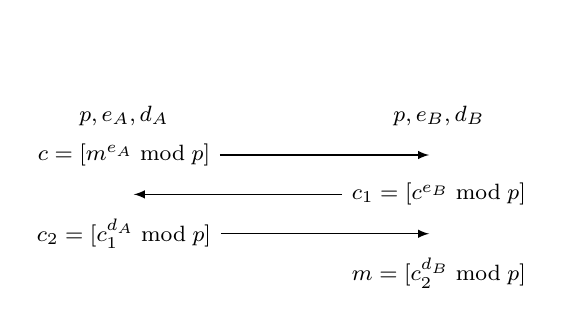
\begin{tikzpicture}[font=\footnotesize]
\node (A) at (0,0) {\Alice};
\node (B) [right of = A, node distance = 4cm] {\Bob};
\node (1a) [below of=A, node distance=1cm] {$p,e_A,d_A$};
\node (1b) [below of=B, node distance=1cm] {$p,e_B,d_B$};
%\draw[-latex] (1a) -- (1b) node [midway,above] {};
\node (2a) [below of=1a, node distance=0.5cm] {$c = [m^{e_A} \bmod p]$};
\node (2b) [below of=1b, node distance=0.5cm] {};
\draw[-latex] (2a) -- (2b) node [midway,above] {};
\node (3a) [below of=2a, node distance=0.5cm] {};
\node (3b) [below of=2b, node distance=0.5cm] {$c_1 = [c^{e_B} \bmod p]$};
\draw[-latex] (3b) -- (3a) node [midway,above] {};
\node (4a) [below of=3a, node distance=0.5cm] {$c_2 = [c_1^{d_A} \bmod p]$};
\node (4b) [below of=3b, node distance=0.5cm] {};
\draw[-latex] (4a) -- (4b) node [midway,above] {};
\node (5a) [below of=4a, node distance=0.5cm] {};
\node (5b) [below of=4b, node distance=0.5cm] {$m=[c_2^{d_B} \bmod p]$};
\end{tikzpicture}
